\def\QRCODE{MASTER_mispa_TUT.IMG.colip_pythonqrcode.png}
\def\QRPAGE{http://www.iptutorials.science/tree/master/MASTER_mispa/TUT.IMG.colip/python}
\pcorrectionsection{Python correction}


\begin{python}
import numpy as np
import matplotlib.pyplot as plt
import skimage.color as color
\end{python}


First of all, the maximal value $M_0$ is arbitrarily fixed at 100.

\begin{python}
def getColipM0():
    # return M0 value
    return 100;
\end{python}

\vspace*{-.3\baselineskip}

\subsection{LMS tones}
This is the difficult part of LIP and CoLIP. Be careful with the use of the function \pinline{eps} that returns the precision at a given double value.
\begin{python}
def lmstone(LMS):
    M0= getColipM0();
    return (M0-np.finfo(float).eps)*(1-LMS/M0);
\end{python}

\vspace*{-.3\baselineskip}

\subsection{Isomorphism}
The isomorphism is the conversion into/back from the logarithmic space.

\begin{python}
def phi(f, M):
    # LIP isomorphism
    # f: graytone function
    # M: maximal value
    l = -M * np.log(-f/M+1);
    return l
\end{python}

\begin{python}
def invphi(l, M):
    # inverse isomorphism
    f = M*(1-np.exp(-l/M));
    return f
\end{python}

\vspace*{-.3\baselineskip}

\subsection{XYZ to LMS}
This conversion uses the HPE matrix (Hunt, Pointer, Estevez).

\begin{python}
def XYZ2LMS(XYZ):
    """
    conversion function
    XYZ: data in XYZ space
    """
    U=np.array([[0.38971, 0.68898, -0.07869],
		[-0.22981,1.18340,  0.04641],
		[0,       0,        1      ]]);
    m, n = XYZ[:,:,0].shape;
    print(m,n)
    XYZ = XYZ.reshape((m*n, 3)).transpose();
    print(XYZ.shape)
    LMS = np.matmul(U, XYZ);
    
    return LMS.transpose().reshape((m, n, 3));
\end{python}

\subsection{Conversions into Colip space}
The conversion into \cargyb  goes first into \targyb. It consists on a conversion matrix followed by the absolute value and the operation to get symmetric channels in the colip space.
\begin{python}
def LMS2ARGYBhat(LMS):
    ARGYBtilde = LMS2ARGYBtilde(LMS);
    return ARGYBtilde2ARGYBhat(ARGYBtilde);
\end{python}

\begin{python}
 def LMS2ARGYBtilde(LMS):
    """
    conversion function
    LMS: data in LMS space
    """
    M0 = getColipM0();
    m, n, p = LMS.shape;
    LMStone = lmstone(LMS);
    LMStilde= phi(LMStone, M0);
    P = [[40/61,20/61,1/61], [1,-12/11,1/11], [1/9,1/9,-2/9 ]];
    
    LMStilde = LMStilde.reshape((m*n, 3)).transpose();
    ARGYBtilde = np.matmul(P, LMStilde).transpose();
    return ARGYBtilde.reshape((m, n, 3));
    \end{python}
    
\begin{python}
def ARGYBtilde2ARGYBhat(ARGYBtilde):
    """
    conversion into ARGYB tilde space
    ARGYBtilde: data in ARGYB tilde space
    
    """
    M0 = getColipM0();
    
    ARGYBhat = np.zeros(ARGYBtilde.shape);
    ARGYBhat[:,:,0] = invphi(ARGYBtilde[:,:,0], M0);
    
    for c in (1,2):
        tmp = np.abs(ARGYBtilde[:,:,c]);
        
        ARGYBhat[:,:,c] = np.sign(ARGYBtilde[:,:,c]) * invphi(tmp, M0);
        
    return ARGYBhat;
    \end{python}


\subsection{CMF}
The color matching functions are provided for convenience. There exist many resources on the internet where they can be found. The classical diagram in the xy space (the horseshoe) is shown in Fig.\ref{fig:colip:python:xy}.

\begin{python}
with np.load('cmf.npz') as data:
    cmap = data['cmap'];
    pourpresLMS = data['pourpresLMS'];
    SpecXYZ = data['SpecXYZ'];
    SpecLMS = data['SpecLMS'];
    SpecRGB = data['SpecRGB'];
    l = data['l'];
    
# display classical CMF in xy
xn = SpecXYZ[:,:,0]/np.sum(SpecXYZ, axis=2);
yn = SpecXYZ[:,:,1]/np.sum(SpecXYZ, axis=2);
zn = 1-xn-yn;
plt.scatter(xn, yn, c=cmap);
\end{python}

\begin{figure}[htbp]
	\centering\caption{Color matching functions in the xy space.}%
	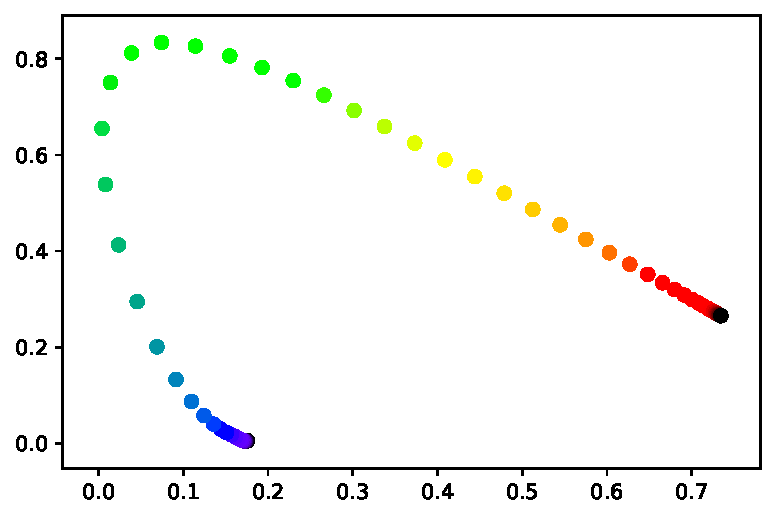
\includegraphics[width=.8\linewidth]{xy.python.pdf}%
	\label{fig:colip:python:xy}%
\end{figure}

To display the CMF and the cube of all RGB colors in the  $(\h{rg},\h{yb})$ space, the following code is used:
The result is shown in Fig.\ref{fig:colip:python:rgyb}.
\begin{python}
#Color matching functions in colip space
ARGYB_hat = LMS2ARGYBhat(SpecLMS);
plt.figure();
plt.scatter(ARGYB_hat[:,0,1], ARGYB_hat[:,0,2], c = cmap);
# purple line
purple_ARGYB_hat = LMS2ARGYBhat(pourpresLMS);
plt.scatter(purple_ARGYB_hat[:,0,1], purple_ARGYB_hat[:,0,2], c='black');
\end{python}

The RGB cube is first generated and then converted into the colip space.
\begin{python}
# number of color in each direction
N=10;
cols = np.linspace(0, 255, num=N);
R, G, B = np.meshgrid(cols, cols, cols);

# reshape the cube for manipulation
R = R.reshape((R.size, 1));
G = G.reshape((G.size, 1));
B = B.reshape((B.size, 1));
NN  = R.size;
colRGB = np.concatenate((R, G, B), axis=1);
cubeRGB = colRGB.reshape((NN, 1, 3));
colRGB = colRGB / 255;

# conversions
cubeXYZ = color.rgb2xyz(cubeRGB);
cubeLMS = XYZ2LMS(cubeXYZ);
cubeARGYBhat = LMS2ARGYBhat(cubeLMS);
plt.scatter(cubeARGYBhat[:,0,1], cubeARGYBhat[:,0,2], c=colRGB);
\end{python}

The color matching functions in the colip space are represented in Fig.\ref{fig:colip:python:rgyb}. A lot could be said about this diagram. For examples, one can notice the approximations in the high (red) wavelengths: this comes from the numerical approximations and the lack of data of the original CMFs. Moreover, the purple line (represented here in black) is not a line in this diagram. This raises the question of the choice of this line in (xy), which was made only by simplicity.

\begin{figure}[htbp]
	\centering\caption{Color matching functions in the $(\h{rg},\h{yb})$ space.}%
	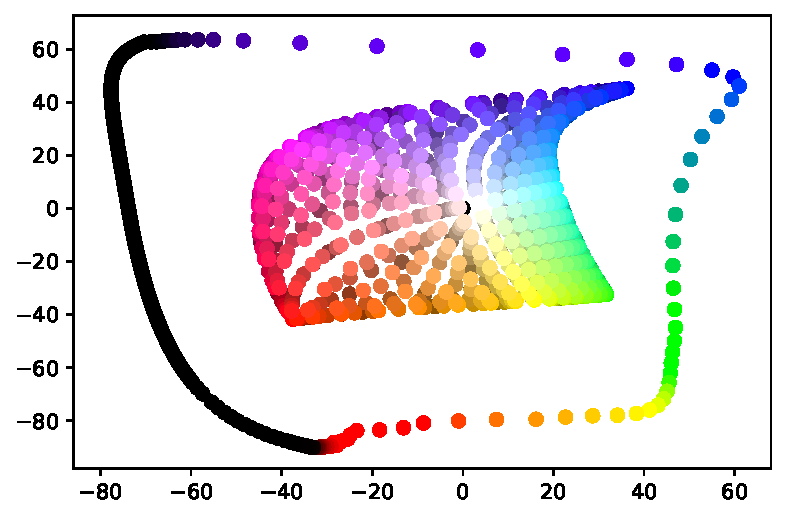
\includegraphics[width=.8\linewidth]{argyb.python.pdf}%
	\label{fig:colip:python:rgyb}%
\end{figure}
